\documentclass[10pt,mathserif]{beamer}

\usepackage[utf8]{inputenc}
\usepackage{parskip}
\usepackage{amsmath}
\usepackage{physics}
\usepackage{stackengine}
\usepackage{float}
\usepackage{cleveref}
\usepackage{graphics}
\usepackage{siunitx}

\allowdisplaybreaks

\newcommand\textbff[1]{\textbf{\boldmath #1}}
\newcommand\circled[1]{\raisebox{.5pt}{\textcircled{\raisebox{-.9pt} {#1}}}
    }
\newcommand{\shortnote}[1]{\textit{\footnotesize (#1)}}

\newcommand{\pp}{\partial}
\newcommand{\mgrad}{\su{\nabla}}

% We often use underlines here
\newcommand\barbelow[1]{\stackunder[1.2pt]{$#1$}{\rule{1.5ex}{.1ex}}}
\newcommand{\su}[1]{\barbelow{#1}}
\newcommand{\du}[1]{\barbelow{\barbelow{#1}}}

\newcommand{\EE}{$\du{E}$}
\newcommand{\PP}{$\du{\Pi}$}
\newcommand{\ddelta}[4]{\delta_{#1#3}\delta_{#2#4} + \delta_{#1#4}\delta_{#2#3}}

\newcommand{\YY}[3][j]{E_{#2#1}E_{#3#1}^*}

\def\onedot{$\mathsurround0pt\ldotp$}
\def\cddot{\mathbin{
    \vcenter{\baselineskip1ex \vspace{-0.1ex}\hbox{\onedot}\hbox{\onedot}}
}}


\begin{document}

\setlength{\abovedisplayskip}{1em}
\setlength{\belowdisplayskip}{0ex}

% \usefonttheme[onlymath]{serif}

\begin{frame}
    % \frametitle{E theory}
    \centering
    \vspace{2em}
    \Large
    Extending a complex tensor model for smectics \\
    \normalsize
    \vspace{0.5em}
    MPhys project 2023/24 \\

    \vspace{2em}

    \emph{Jan Kocka} \\
    \footnotesize supervised by \emph{Dr Tyler N Shendruk}

    \vspace{3em}

    \small
    Two main goals: adapt it for 3D \hspace{1ex}\&\hspace{1ex} introduce projection operators to free energy terms
    % adapting for 3D \hspace{1em}\&\hspace{1em} introducing projection operators to grad
\end{frame}

\begin{frame}
    \frametitle{Smectic liquid crystals}
    \begin{columns}
        \begin{column}{0.49\textwidth}
            \begin{itemize}
                \item Layering of long molecules \color{gray} (simplest case) \normalcolor
                \item Smectic A -- molecules perpendicular to layers
                \item 3 quantities \color{gray} (fields) \normalcolor
                    \begin{itemize}
                        \item How ordered the phase is
                        \item Direction of layering -- director $\su{N}$
                        \item Spacing of layers
                    \end{itemize}
            \end{itemize}
        \end{column}
        \begin{column}{0.49\textwidth}
            \begin{figure}
                \centering
                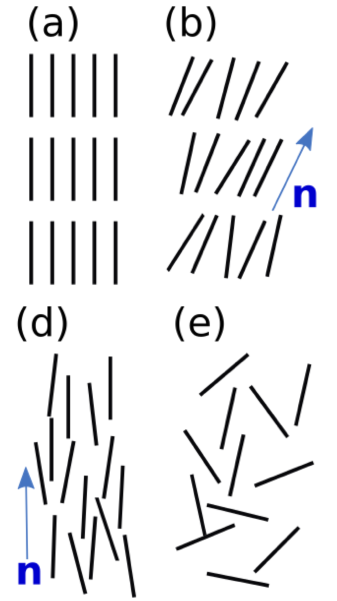
\includegraphics[width=0.5\textwidth]{figures/phases.pdf}
                \caption{Crystaline, smectic C, nematic and isotropic phases}
            \end{figure}
        \end{column}
    \end{columns}
\end{frame}

\begin{frame}
    \frametitle{Describing smectics}
    \begin{itemize}
        \item The layering is a density fluctuation
    \end{itemize}
    \begin{align*}
        \rho(\su{r}, t) = \sum_{m=-\inf}^{+\inf} \psi_m e^{im\su{q}\cdot\su{r}} \simeq \rho_0 + 2\Re(\psi e^{i\su{q_0}\cdot\su{r}})
    \end{align*}
    \begin{itemize}
        \item Having $\psi = |\psi|e^{i\phi}$ gives
            \begin{itemize}
                \item $|\psi|$ as the order parameter
                \item Changes in $\phi$ lead to spacing differences
            \end{itemize}
        \item $\su{N} \propto \su{q_0}$ \color{gray}, can be an additional parameter or taken as $\su{\nabla} \phi$ \normalcolor
    \end{itemize}
\end{frame}

\begin{frame}
    \frametitle{E theory}
    \begin{itemize}
        \item Inspiration from Q-tensor and complex $\psi$
    \end{itemize}
    \begin{align*}
        \du{Q} &= S_1(\su{N}\su{N} - \frac{\du{\delta}}{d}) \qq{\color{gray} uniaxial case \normalcolor}
    \end{align*}
    \begin{itemize}
        \item Replace the real order parameters $S$ with complex $\psi$
    \end{itemize}
    \begin{align*}
        \du{E} &\sim \psi_1(\su{N}\su{N} - \frac{\du{\delta}}{d})
    \end{align*}
    \begin{itemize}
        \item Incorporates $\su{N} \leftrightarrow -\su{N}$ symmetry
        \item One object -- allows numerical melting
        \item $\su{N}$, $|\psi|$ and $\arg(\psi)$ are separate degrees of freedom
    \end{itemize}

    \vspace{1ex}
    \small \color{gray} $d$ is the number of dimensions, 2 or 3 \normalcolor
\end{frame}

\begin{frame}
    \frametitle{E theory numerics}
    \begin{align*}
        \du{E} &\sim \psi_1(\su{N}\su{N} - \frac{\du{\delta}}{d})
    \end{align*}
    \begin{itemize}
        \item Want to evolve \EE\ directly as a $d\text{x}d$ complex tensor
        \item Enforce the form above?
        \item Inspiration from $\du{Q}$ -- symmetric and traceless 
        \begin{itemize}
            \item real so can be diagonalized
        \end{itemize}
        \item Require $\du{E}$ be unitarily diagonalizable (normal), symmetric and traceless
    \end{itemize}
\end{frame}

\begin{frame}
    \frametitle{Constraints on E}
    Leads to the following form in 3D \color{gray} (equivalent in 2D, but only 1 term) \normalcolor
    \begin{align*}
        \du{E} &= \du{U}^\dagger \begin{pmatrix}
            \lambda_1 & 0 & 0 \\
            0 & \lambda_2 & 0 \\
            0 & 0 & - \lambda_1 - \lambda_2
        \end{pmatrix} \underset{\text{also using symmetry}}{\du{U} = \cdots = \psi_1(\su{N}}\su{N} - \frac{\du{\delta}}{3}) + \psi_2(\su{M}\su{M} - \frac{\du{\delta}}{3})
    \end{align*}
    \begin{itemize}
        \item With $\su{N}$, $\su{M}$ being real, orthogonal, unit vectors, and
    \end{itemize}
    \begin{align*}
        \begin{pmatrix} \psi_1 \\ \psi_2 \end{pmatrix} = \begin{pmatrix} 2 & 1 \\ 1 & 2 \end{pmatrix} \begin{pmatrix} \lambda_1 \\ \lambda_2 \end{pmatrix} = \begin{pmatrix} \lambda_1 - \lambda_3 \\ \lambda_2 - \lambda_3 \end{pmatrix}
    \end{align*}
    \begin{itemize}
        \item \color{gray} so the $\psi$s are the differences from the third eigenvalue\normalcolor
        \item Clearly biaxial form of the E we want!
    \end{itemize}
\end{frame}

\begin{frame}
    \frametitle{Biaxial E}
    \begin{itemize}
        \item Theory suggests a biaxial E in 3D
        \item Perpendicular layering?
        \begin{itemize}
            \item Happens at interfaces in numerics -- we get similar features to other studies using a tetratic order parameter
        \end{itemize}
        \item No clear constraint to force it uniaxial
    \end{itemize}
\end{frame}

\begin{frame}
    \frametitle{E theory -- Ginzburg-Landau}
    \begin{itemize}
        \item Dynamics using Ginzburg-Landau theory
        \item Need a free energy in terms of \EE
        \item Use $\pdv{E_{ij}}{t} = -\mu\fdv{F}{E_{ij}^*}$ \color{gray} + Lagrange multipliers for constraints \normalcolor
    \end{itemize}
\end{frame}

\begin{frame}
    \frametitle{The free energy -- bulk}
    \begin{itemize}
        \item $F$ must be real -- need to match $\du{E}$ and $\du{E}^*^$, simplest is
    \end{itemize}
    \begin{align*}
        f_\text{bulk}(E_{ij}E_{ij}^* = \Tr(\du{E}\du{E}^*)) = \frac{A}{2} E_{ij}E_{ij}^* + \frac{C}{4} (E_{ij}E_{ij}^*)^2
    \end{align*}
    \begin{itemize}
        \item \color{gray} In the uniaxial case $E_{ij}E_{ij}^* \propto |\psi|^2$ \normalcolor
    \end{itemize}
\end{frame}

\begin{frame}
    \frametitle{The free energy -- elastic terms}
    \vspace{1em}
    \begin{itemize}
        \item Need gradients
        \item Take all to be of form $|?|^2$ \color{gray} (Frobenius norm) \normalcolor
        \item Only allow a single \EE, and 1 or 2 $\su{\nabla}$
    \end{itemize}
    \begin{align*}
        &|\su{\nabla}\du{E}|^2 = E_{ij,k}E_{ij,k}^* \qq{Simplest term} \\
        &|\su{\nabla}\cdot\du{E}|^2 = E_{ij,j}E_{ik,k}^* \qq{Divergence like, new} \\
        \\
        &|\nabla^2\du{E}|^2 = E_{ij,kk}E_{ij,ll}^* \qq{Simplest double gradient, considered}
    \end{align*}
\end{frame}

\begin{frame}
    \frametitle{Projection operators for $F$}
    \begin{itemize}
        \item Gradients in different directions have different energy costs
        \item For \textbf{uniaxial} \EE, special direction is $\su{N}$
        \item Projection operator $\du{\Pi}=\su{N}\su{N}$, rest is $\du{T} = \du{\delta} - \du{\Pi}$
        \item Consider $\su{\nabla} \rightarrow a \du{\Pi}\cdot\su{\nabla} + b \du{T}\cdot\su{\nabla}$ \color{gray} $a, b$ being some constants \normalcolor
    \end{itemize}

    \begin{align*}
        &E_{ij,k}E_{ij,k}^* \rightarrow f_\text{comp} = b_1^\parallel \Pi_{kl} E_{ij,k}E_{ij,l}^* + b_1^\perp T_{kl} E_{ij,k}E_{ij,l}^* \\
        &E_{ij,kk}E_{ij,ll}^* \rightarrow f_\text{curv} = b_2^\parallel \Pi_{kl}E_{ij,lk}\Pi_{mn}E_{ij,nm}^* + b_2^\perp T_{kl}E_{ij,lk}T_{mn}E_{ij,nm}^* \\
        &\phantom{E_{ij,kk}E_{ij,ll}^* \rightarrow f_\text{curv} =}+ b_2^{\parallel\perp}(\Pi_{kl}E_{ij,lk}T_{mn}E_{ij,nm}^* + T_{kl}E_{ij,lk}\Pi_{mn}E_{ij,nm}^*)
    \end{align*}
\end{frame}

\begin{frame}
    \frametitle{Projection operators}
    \begin{itemize}
        \item Need a form for \PP\ in terms of \EE
        \item Have 2 forms which work for uniaxial \EE
    \end{itemize}
    \begin{align*}
        \du{\Pi} =& \sqrt{\frac{d-1}{d \du{E} \cddot \du{E}}} \du{E} + \frac{\du{\delta}}{d} \\
        \du{\Pi} =& \frac{d-1}{d-2}\qty(\frac{\du{E} \cdot \du{E}^*}{\du{E} \cddot \du{E}^*} - \frac{\du{\delta}}{d(d-1)})
    \end{align*}
    \begin{itemize}
        \item First is significantly easier to work with
        \color{gray}
        \item Lead to seemingly different functional derivatives -- why?
        \item First form only has $\du{E}$, how about $\du{E} \rightarrow \du{E}^*$?
        \item How well do they work for biaxial \EE?
        \normalcolor
    \end{itemize}
\end{frame}

\begin{frame}
    \frametitle{Functional derivatives using \PP}
    \begin{itemize}
        \item Results using the square root version of \PP
    \end{itemize}
    \small
    \begin{align*}
        \fdv{F_\text{bulk}}{E_{ij}^*} =&\enspace \frac{1}{2}\qty(A + C E_{ab}E_{ab}^*)E_{ij} \\
        \fdv{F_\text{comp}}{E_{ij}^*} =&\enspace -(b_1^\parallel - b_1^\perp) (\Pi_{kl,l} E_{ij,k} + \Pi_{kl} E_{ij,kl}) - b_1^\perp E_{ij,kk} \\
        \fdv{F_\text{curv}}{E_{ij}^*} =&\enspace (b_2^\parallel + b_2^\perp - 2b_2^{\parallel\perp}) \Bigl( (\Pi_{kl}\Pi_{po,po} + 2\Pi_{kl,o}\Pi_{po,p} + \Pi_{kl,po}\Pi_{po})E_{ij,lk} \\
        &\phantom{\enspace (b_2^\parallel + b_2^\perp - 2b_2^{\parallel\perp}) \Bigl(}+ 2(\Pi_{kl,o}\Pi_{po} + \Pi_{kl}\Pi_{po,o})E_{ij,lkp} + \Pi_{kl}\Pi_{po}E_{ij,lkpo} \Bigr) \nonumber \\
        &+ (b_2^{\parallel\perp} - b_2^\perp)\Bigl( \Pi_{po,po}E_{ij,kk} + 2\Pi_{po,o}E_{ij,kkp} + \Pi_{po}E_{ij,kkpo} \nonumber \\ 
        &\phantom{\enspace+ (b_2^{\parallel\perp} - b_2^\perp)\Bigl(}+ \Pi_{kl,oo}E_{ij,lk} + 2\Pi_{kl,o}E_{ij,lko} + \Pi_{kl}E_{ij,lkoo} \Bigr) \nonumber \\ 
        &+ b_2^\perp E_{ij,kkoo} \nonumber
    \end{align*}
\end{frame}

\begin{frame}
    \frametitle{Lagrange multipliers}
    \begin{itemize}
        \item Back to enforcing the constraints
    \end{itemize}
    \begin{align*}
        \qq{Minimize} \int \Bigl(f(\du{E}, \su{\nabla}\du{E}, \ldots) + \lambda_s g_s(\du{E}) + \lambda_t g_t(\du{E}) + \lambda_n g_n(\du{E})\Bigr) \dd{V}
    \end{align*}
    \begin{itemize}
        \item Need real, non-negative $g_?(\du{E})$ that reflect the constraints:
    \end{itemize}
    \begin{align*}
        g_s &= |E_{ij} - E_{ji}|^2 \\
        g_t &= |E_{ii}|^2 \\
        g_n &= |E_{ik}E_{kj}^* - E_{ik}^*E_{kj}|^2
    \end{align*}
    \begin{itemize}
        \item Decide what to use for $\lambda$s -- analytic guess, soft constraints etc.
    \end{itemize}
\end{frame}

\begin{frame}
    \centering
    \Large
    Thank you for your attention
\end{frame}

\begin{frame}
    \frametitle{Gradients of \PP}
    \begin{itemize}
        \item Results using the square root version of \PP
    \end{itemize}
    \begin{align*}
        \Pi_{kl} =&\enspace \frac{s E_{kl}}{\sqrt{E_{ab}E_{ab}}} + \frac{\delta_{kl}}{d} \\
        \Pi_{kl,m} =&\enspace \frac{s}{\sqrt{E_{ab}E_{ab}}} \qty(E_{kl,m} - \frac{E_{kl}E_{cd}E_{cd,m}}{E_{ab}E_{ab}}) \\
        \Pi_{kl,mn} =&\enspace \frac{s}{\sqrt{E_{ab}E_{ab}}} \Biggl(E_{kl,mn} \\ 
        &-\frac{E_{kl,n}E_{cd}E_{cd,m} + E_{kl,m}E_{cd}E_{cd,n} + E_{kl}(E_{cd,n}E_{cd,m} + E_{cd}E_{cd,mn})}{E_{ab}E_{ab}} \\
        &\phantom{\frac{s}{\sqrt{E_{ab}E_{ab}}} \Biggl(} + 3\frac{E_{kl}E_{cd}E_{cd,m}E_{ef}E_{ef,n}}{(E_{ab}E_{ab})^2} \Biggr)
    \end{align*}
\end{frame}

\end{document}
